\chapter{ラップタイムの評価方法}
\label{chap:method}
本章では，ラップタイムを要素別の時間差に分解する方法，評価に必要な車両応答と経路生成の誤差の同定方法，および要素ごとの比較に用いる閉ループシミュレーションの構成を述べる．

\section{ラップタイムの内訳}
\label{sec:decomposition}
実測のラップタイム$T_{\mathrm{lap}}$を，走行した軌跡の上で速度列を順に置き換えたときの時間差の和として表す．
\begin{equation}
  T_{\mathrm{lap}} = T_{\mathrm{phys}} + \Delta T_{\mathrm{cap}} + \Delta T_{\mathrm{plan}} + \Delta T_{\mathrm{path}} + \Delta T_{\mathrm{track}} + \Delta T_{\mathrm{stop}}
  \label{eq:decomp}
\end{equation}
走行した軌跡の弧長を$s$（車輪速度の積算による），軌跡の曲率を$\kappa(s)$とし，ある速度列$v(s)$による所要時間を$T[v]=\int ds/v(s)$と書く．停止点が発行されてから速度が計画値に戻るまでの区間を停止イベントの窓$W$（以下，停止窓）と呼び（停止点が最初に発行された時刻から，最後の発行の1\,s後以降に実測速度の0.3\,s移動平均が窓の直前の計画速度$v_b$の95\%に戻る時刻まで），それ以外の走行区間を移動区間と呼ぶ．各項は次のように定義する．
\begin{description}[leftmargin=2\zw]
  \item[$T_{\mathrm{phys}}$（基準時間）] 車両の物理的な限界だけを与えた速度列$v_{\mathrm{phys}}(s)$による時間$T[v_{\mathrm{phys}}]$．物理的な限界とは，走行可能な上限速度（従動輪のシミー（自励的な首振り振動）が6.5\,m/sで発散したため，余裕を見て6.0\,m/s），同定した加速と減速の上限，手動走行で観測した横加速度の最大値（5〜7\,m/s$^2$）に基づく横加速度の上限6.0\,m/s$^2$である．速度列は，各点の上限$\min(v_{\max},\sqrt{a_{y,\max}/|\kappa|})$に対して，\eqnref{eq:forward}と\eqnref{eq:backward}を加速側と減速側に走査して求める．
  \item[$\Delta T_{\mathrm{cap}}$（上限速度の設定による時間差）] 上の速度列にソフトウェアの上限速度$v_{\mathrm{cap}}$を加えた速度列$v_{\mathrm{ref}}(s)$による時間$T_{\mathrm{ref}}=T[v_{\mathrm{ref}}]$と$T_{\mathrm{phys}}$の差．
  \item[$\Delta T_{\mathrm{plan}}$（速度計画の設定値による時間差）] 同じ軌跡に速度計画の設定値（$a_{y,\max}=3.0$，$a_{x,\max}=3.0$\,m/s$^2$，$v_{\mathrm{cap}}$）を与えた速度列$v_{\mathrm{plan}}(s)$による時間と$T_{\mathrm{ref}}$の差．速度計画の設定値が物理限界に対して持つ余裕を表し，記録された設定値が物理限界より大きい場合は負になる．
  \item[$\Delta T_{\mathrm{path}}$（経路生成による時間差）] 記録された速度計画の出力を，制御器と同じく自車位置の0.3\,s先の点で参照した速度列$v_{\mathrm{rec}}(s)$による時間と$T[v_{\mathrm{plan}}]$の差．制御器が実際に参照した速度を用いることで，次の$\Delta T_{\mathrm{track}}$が追従の遅れだけを表すようにする．速度計画の設定値が同じであるから，両者の差は速度計画に入力された経路（経路生成と平滑化の出力）と走行軌跡の違い，すなわち曲率の誤差と認識距離の不足に起因する．平滑化後の経路が曲率を過小に評価すると計画速度は走行軌跡上の値より高くなるため，この項は負になりうる．なお，経路選択の指示に応じて速度計画の上限が変わる分岐での速度抑制は，記録された出力にのみ含まれるため，計算上はこの項に入る．結果ではその分を分けて示す．
  \item[$\Delta T_{\mathrm{track}}$（経路追従による時間差）] 移動区間における，実測速度による時間$T[v_{\mathrm{meas}}]$と$T[v_{\mathrm{rec}}]$の差．追従制御の遅れと，追従誤差に伴う減速を表す．
  \item[$\Delta T_{\mathrm{stop}}$（停止による時間差）] 停止イベントの窓について，実測の経過時間と，窓内の走行距離$d_W$を窓の直前の計画速度$v_b$で通過した場合の時間$d_W/v_b$との差．
\end{description}
窓の内側では，$v_{\mathrm{plan}}$と$v_{\mathrm{rec}}$を$v_b$で置き換える．したがって$\Delta T_{\mathrm{plan}}$と$\Delta T_{\mathrm{path}}$は窓の内側では0であり，窓の内側の実測時間と$d_W/v_b$の差はすべて$\Delta T_{\mathrm{stop}}$に入る．このように各項は同じ軌跡の上で速度列を順に置き換えた時間差であるから，その和は恒等的に$T_{\mathrm{lap}}$に一致する（数値計算上の差は$10^{-4}$\,s未満）．残差は分解の妥当性を示す量にはならず，分解に用いる車両モデルの妥当性は\ref{sec:sil}節の閉ループシミュレーションの予測誤差で別に示す．また，置き換えの順序や参照点の取り方を変えると隣り合う項のあいだで値の配分が変わる．本論文では上の順序に固定し，参照点，曲率の平滑化，窓の終端の判定を変えたときの感度を併記する．記録データから計算できない，記録に存在しない仮想的な条件（例えば追従が理想であった場合の実測速度）は扱わない．

軌跡の曲率は，慣性航法装置のヨーレート$r$と実測速度$v$から$\kappa=r/v$として求め，走行距離に対して幅（$\sigma$）1.0\,mのガウス平滑をかける．各項は符号付きで示し，コースを直線とカーブ（$\sigma=1.5$\,mで平滑した曲率で$|\kappa|>0.04$\,1/m）に分けた区間ごとにも集計する．区間ごとの値は前の区間の出口速度に依存するため，互いに独立な量ではない．

この分解の限界として，基準時間は実際に走行した軌跡の上で定義するため，追従誤差による経路長と曲率の増加が$T_{\mathrm{phys}}$に含まれる．

\section{車両応答の同定}
\label{sec:identification}
基準時間と閉ループシミュレーションに用いる車両モデルは，実車の走行記録から同定する．同定するのは次の4つである．
\begin{enumerate}
  \item 並進速度の指令値に対する実速度の応答：むだ時間と一次遅れ，定常ゲイン，加速と減速それぞれの上限．
  \item 舵角の指令値に対するヨーレートの応答：ヨーレートと速度から等価舵角$\delta_{\mathrm{eq}}=\arctan(L r / v)$を求め，むだ時間と一次遅れ，ゲインとして当てはめる．ここで$L$はホイールベース，$r$はヨーレート，$v$は並進速度である．
  \item 従動輪の実舵角と等価舵角の関係：従動輪の舵角から車体のヨー運動がどの程度決まるかを表す．
  \item 認識から指令までの遅延：画像の撮影時刻と，その画像に基づく経路が制御に使われた時刻の差．
\end{enumerate}
入力はジョイスティックによる手動の段階入力とパルス入力，および自律走行中の指令と応答を用いる．同定に用いた走行と検証に用いた走行は分ける．

\section{経路生成の誤差の計測}
\label{sec:path_error}
経路生成の誤差は，閉ループシミュレーションで経路生成を置き換えるモデルに用いる．記録した画像に対する推論結果について，次の量を求める．
\begin{enumerate}
  \item 前方距離ごとの横位置の誤差：前後1\,sの推論結果を自己位置推定の変位で現在の車両座標系に揃えた中央値を基準とし，各フレームの横位置との差を，前方距離ごとに集計する．
  \item 経路生成の出力が得られている前方距離（\ref{sec:path_smoother}節の認識距離）の分布．
  \item 交差点手前での進行方向ごとの経路の分離．
\end{enumerate}
路面に対する絶対的な誤差は，GNSSの参照位置とベクターマップの車線中心に対して求める．3次元LiDAR等による独立した参照は本研究では取得していない．

\section{閉ループシミュレーション}
\label{sec:sil}
要素ごとの比較は，実車で動作しているソフトウェアをそのまま用いた閉ループシミュレーション（software-in-the-loop simulation．以下，実装SIL）で行う．Fig.~\ref{fig:sil}に構成を示す．経路の平滑化，局所経路計画，速度計画，経路追従制御の各ノードは実装をそのまま実行し，車両と経路生成，信号・障害物の検出をモデルで置き換える．

\begin{figure}[H]
  \centering
  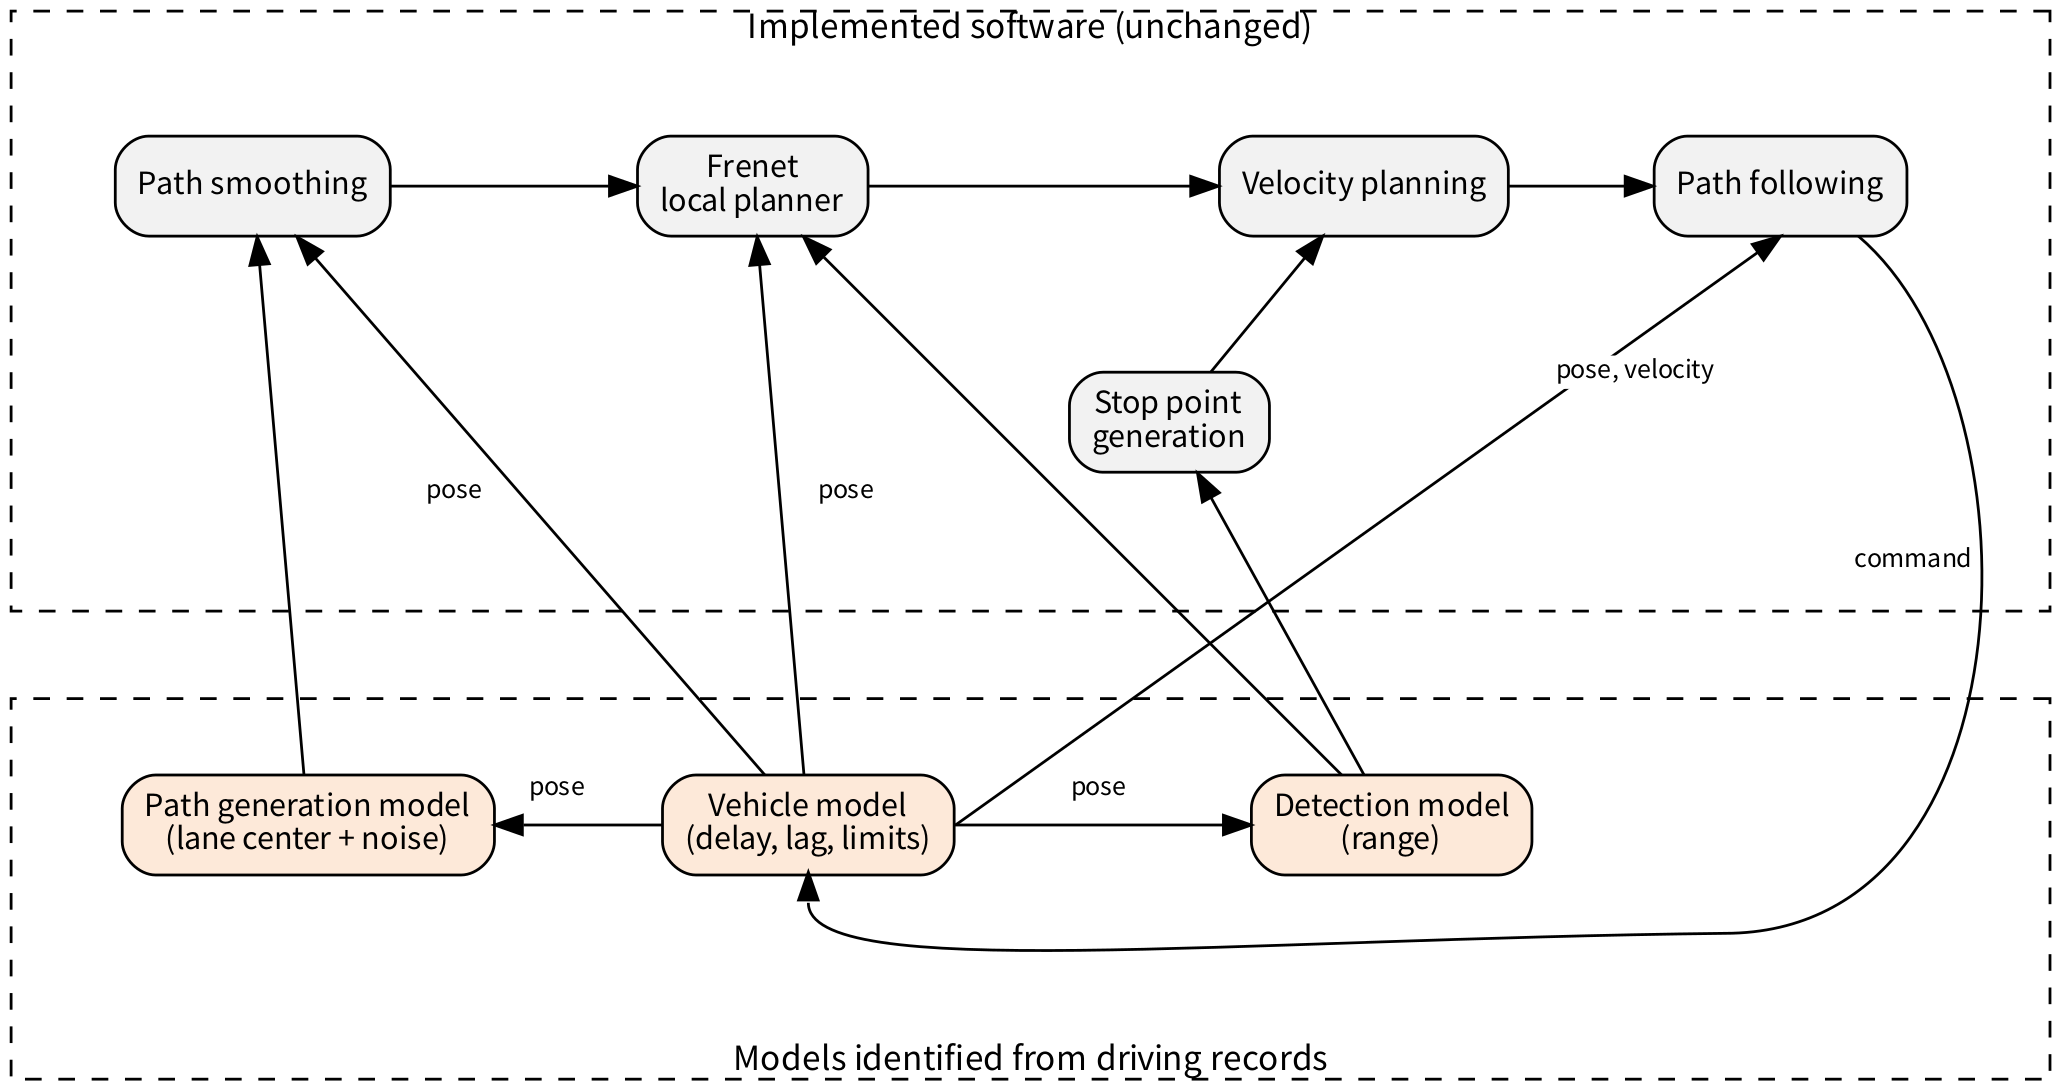
\includegraphics[width=\textwidth]{images/sil.png}
  \caption{Configuration of the closed-loop simulation. The implemented software (path smoothing, Frenet local planner, velocity planning, path following, and stop point generation) is run unchanged; the vehicle, the path generation, and the detection are replaced by models identified from the driving records.}
  \label{fig:sil}
\end{figure}

\subsection{車両モデル}
並進速度は，\ref{sec:identification}節で同定したむだ時間と一次遅れ，加速・減速の上限で表す．舵角は，指令値に対するむだ時間と一次遅れ，ゲインで表し，$\pm 15^\circ$で制限する．ゲイン0.92は10月12日の記録から得た値であり，Table~\ref{tab:ident}の約1.0（等価舵角の応答，3\,m/s以上）とは当てはめの対象と条件が異なる．ヨーレートは等価舵角と速度から求める．横加速度が摩擦限界を超える分は曲がれないものとし，ヨーレートを$\mu g/v$（$\mu g$は摩擦限界の横加速度）で飽和させる．

\subsection{経路生成のモデル}
経路生成は，コースの車線中心から車両前方の一定距離（認識距離）までを切り出し，\ref{sec:path_error}節で計測した誤差の分布に従う雑音を加えて経路生成の出力（目標経路）とする（記録から求めた経路生成の誤差特性．以下，実測誤差モデル）．雑音は前方距離ごとに大きさを変え，経路の先端ほど大きくする．認識距離は一定（9\,m）とし，実測誤差モデルの条件では1割のフレームで経路が5.8\,mで途切れる．経路生成の出力は前方距離ごとの点（行）の列であり，実測誤差モデルの行は0.77〜8.89\,mの21点で，5\,m以遠には5.83\,mと8.89\,mの2点しか持たない（以下，この行の並びを行構成と呼ぶ）．行構成を0.5\,m間隔（0.8〜8.8\,m，17行）にした条件を密な行と呼ぶ．基準の条件では，カーブで認識距離が短くなる効果は経路の切り出しに入れていない．5章では，この効果を入れる条件として，前方6\,m以内にカーブ（$|\kappa|>0.04$\,1/m）があるフレームで6\,m以遠の点を消し，それ以外は9\,mとする条件（6/9\,m切替）も用いる．実測誤差モデルの行では，6/9\,m切替で欠けるのは最遠の8.89\,mの1点だけである（認識距離を4.5\,mに短縮する4.5/9\,m切替では，5.83\,mと8.89\,mの2点が欠ける）．交差点では，経路選択の指示に応じて分岐側の車線中心に切り替える．経路生成の雑音を加えない条件（理想的な経路生成）も比較の端点として用いる．さらに，悲観的な経路生成として，実測の雑音に加えて，自車近傍の接線からの横位置の偏差に$1/(1+(x/8)^2)$（$x$は前方距離）を掛け，遠方の曲率を小さく出す．ここで曲率比とは，ある前方距離で経路（経路生成の出力または平滑化後の経路）から求めた曲率を，実際に走行した曲率で割った値であり，1より小さいほど曲率を小さく見積もっていることを表す．この条件の曲率比は2.5，4，6\,m先で0.44，0.47，0.46であり，10月12日の記録（9月27日版の重み）で得た0.49，0.47，0.41（\ref{sec:horizon_result}項）に合わせたもので，記録の2次平滑化後の曲率比に合わせたものであり，10月24日版の重みでの値ではない．この悲観的な経路生成（以下，悲観モデル）は，10月24日の報告の式を実装SILに再実装したものであり，当時の実装とは別のSILである．さらに，雑音の大きさを実測誤差モデルの0.5倍，2倍にした条件と，認識距離9\,m一定の条件で平滑化の出力を18\,mから9\,mに打ち切る条件（9\,m以遠の外挿部を速度計画と局所経路計画に渡さない．6/9\,m切替との組合せは未実施）も用いる．

\subsection{信号と障害物のモデル}
信号パネルとコーンは，検出できる最遠距離（コーン9.3\,m，パネル20\,m）とカメラの画角（半角55$^\circ$）の内側で検出されるものとし，位置の誤差は入れず，信号の色の誤判定を1フレームあたり3\%の確率で与える．コーンの最遠検知距離9.3\,mは，追試で調整した値ではなく，10月12日の走行記録で信号のコーンが最初に検出された距離（3回の接近で推定距離9.0〜9.5\,m）から定めたSILの検出モデルの既定値であり，パネルは約19\,mで検出できた（距離推定は不安定）．停止点はコーンの3.3\,m手前に発行されるため，停止点までの距離は検知距離から3.3\,mを引いた6.0\,m（検知距離15\,mで11.7\,m，20\,mで16.7\,m）であり，4章の実車で停止点が最初に発行された距離（10月12日で5.3\,m，R2で6.98\,m）の間にある．SILでは検知範囲内（0.8\,m以遠，検知距離の内側，画角の半角55$^\circ$以内）のコーンを毎フレーム位置誤差なしで検出し，揺らぎ・距離の誤差・欠落は入れていない（入れているのは赤パネルの色の入れ替え1フレーム3\%のみ）．速度計画は認識上の距離に基づいて動くため，計画の挙動の再現としては妥当であるが，実車の真の距離は，10月12日の停止3で約11.5\,mと見積もられ（\ref{sec:stop_result}項），SILの約6\,mより長い可能性がある．検知距離15\,m，20\,mの条件は，実車の認識性能の予測ではなく改善案の感度分析である．検出結果に対する停止点の発行と障害物回避は実装をそのまま動かす．

閉ループシミュレーションの主なパラメータをTable~\ref{tab:sil_params}に示す（評価の行は5章の主な比較の条件であり，信号停止の走行は$s=165$\,mまでで打ち切り，日をまたぐ比較は3周，停止の機構の追跡は3シードで行った）．本論文のシミュレーションには，実装ソフトウェアをそのまま動かすもの（実装SIL）と，同じ処理の流れをPythonで再現した簡易モデルがあり（\ref{chap:contribution}章），値が異なる項目は両方の列に示す．車両モデルの並進速度の応答は，10月12日の手動走行をむだ時間0.06\,sと一次遅れ0.60\,sで当てはめた値であり，Table~\ref{tab:ident}の同定値（むだ時間0.20〜0.27\,s，一次遅れ0.39〜0.65\,s）とはモデルの構造が異なるが，両者の合計はほぼ等しい．加速の上限2.5\,m/s$^2$と減速の上限3.5\,m/s$^2$は，同じ記録の保守側の当てはめである．この違いが結果に与える影響は\ref{sec:limitations}節で述べる．

\begin{table}[!t]
  \centering
  \caption{Parameters of the closed-loop simulation.}
  \label{tab:sil_params}
  \scriptsize
  \setlength{\tabcolsep}{4pt}
  \begin{tabular}{L{3.4cm}L{4.4cm}L{7.6cm}}
    \toprule
    項目 & 簡易モデル & 実装SIL \\
    \midrule
    \multicolumn{3}{l}{\textbf{車両モデル}} \\
    並進速度のむだ時間 & 0.06\,s & 0.06\,s \\
    並進速度の一次遅れ & 0.4\,s & 0.60\,s \\
    並進速度の定常ゲイン & 0.97 & 0.965 \\
    加速の上限 & なし & 2.5\,m/s$^2$ \\
    減速の上限 & なし & 3.5\,m/s$^2$ \\
    操舵のむだ時間 & 0.06\,s & 0.06\,s \\
    操舵の時定数 & 0.35\,s & 0.17\,s \\
    操舵のゲイン & 0.9 & 0.92 \\
    舵角の制限 & $\pm 15^\circ$ & $\pm 15^\circ$ \\
    摩擦限界の横加速度 & なし（記録のみ） & 6\,m/s$^2$（超える分は曲がれない） \\
    ホイールベース & 0.733\,m & 0.733\,m \\
    \midrule
    \multicolumn{3}{l}{\textbf{経路生成のモデル}} \\
    認識距離 & 一定9.0\,m（0.8〜9.0\,mに21行） & 一定9.0\,m．実測誤差モデルでは最遠点が8.9\,mで，1割のフレームで欠落（経路長5.8\,m）．変種：6/9\,m切替，密な行（0.5\,m間隔17行） \\
    横位置の誤差（近傍） & 自己相関付きの雑音（$\sigma=0.03$\,m，$\rho=0.955$）と白色雑音0.03\,m & 同左．実測誤差モデルの条件では，全行共通のラプラス分布（尺度0.05\,m，$\rho=0.65$）と白色雑音0.01\,m \\
    横位置の誤差（先端） & $\sigma(x)=0.03+0.045\max(x-2,0)$\,m（9\,mで0.345\,m） & 同左．実測誤差モデルの条件では，最遠の1点にラプラス分布（尺度0.25\,m，$\rho=0.7$）を加算 \\
    画角 & 考慮しない & 半角55$^\circ$を信号とコーンの検出に適用（経路の切り出しには適用しない） \\
    理想 & 雑音なし & 雑音なし，認識距離20\,m，平滑化を経由せず局所経路計画へ入力 \\
    実測 & 上記の距離比例の雑音 & 上記の距離比例の雑音，または実測誤差モデル \\
    悲観 & 実測の雑音に加え，接線からの横位置の偏差に$1/(1+(x/8)^2)$を掛ける & 同左（10月24日の報告の式の再実装） \\
    雑音の倍率 & 同じ倍率（0.5倍，2倍）を掛ける & 実測誤差モデルの全雑音に同じ倍率（0.5倍，2倍）を掛ける \\
    平滑化出力の打切り & -- & 認識距離9\,m一定で出力長を18\,mから9\,mに打ち切る（9\,m以遠の外挿部を渡さない） \\
    \midrule
    \multicolumn{3}{l}{\textbf{検出モデル}} \\
    コーンの最遠検知距離 & 含まない & 9.3\,m \\
    信号パネルの最遠検知距離 & 含まない & 20\,m \\
    検出位置の誤差 & 含まない & 含まない \\
    信号の色の誤判定 & 含まない & 3\%（1フレームごと） \\
    \midrule
    \multicolumn{3}{l}{\textbf{処理周期と遅延}} \\
    経路生成 & 15\,Hz & 15\,Hz \\
    局所経路計画 & 10\,Hz & 10\,Hz \\
    速度計画 & 10\,Hz（局所経路計画と同時） & 局所経路の更新ごと（10\,Hz） \\
    追従制御 & 20\,Hz & 20\,Hz \\
    車両の更新 & 100\,Hz & 100\,Hz \\
    認識から制御までの遅延 & \multicolumn{2}{p{10.8cm}}{撮影から経路生成の出力まで0.06\,s．以降は各処理の周期で生じる（実測は0.106\,s，Table~\ref{tab:ident}）} \\
    \midrule
    \multicolumn{3}{l}{\textbf{評価}} \\
    シード数 & 4 & 5 \\
    乱数化の対象 & 経路生成の雑音の系列 & 経路生成の雑音の系列，信号の色の誤判定 \\
    1回の走行 & 1.02周 & 2周（完走判定は2周で最大横偏差1.5\,m以内） \\
    完走の判定 & 横偏差が1.5\,mを超えた時点で打ち切り，失敗とする & 最大横偏差が1.5\,m以内．2.5\,mを超えた時点で打ち切り \\
    \bottomrule
  \end{tabular}
\end{table}

\subsection{妥当性の確認}
閉ループシミュレーションが実車の走行を再現できることを，次の5つで確認する．第一に，記録した入力（経路生成の出力，自己位置）をシミュレーションに与え，局所経路計画と速度計画の出力が記録と一致することを確かめる．第二に，実車で生じた信号停止での停止位置の行き過ぎ（停止線を越えた量を正とする）を，同定値の範囲内の車両モデルで再現する．第三に，隣接車線への移動を，記録した認識結果と外乱を与えて閉ループで再現する．第四に，10月12日の走行と同じ構成で周回を走行させ，ラップタイムと完走を実車と比較する．第五に，10月12日の記録から同定した車両モデルのまま10月27日の走行の構成で走行させ，日をまたいだ予測を検証する．実車で完走した条件が十分にある場合は，さらに，シミュレーションのラップタイムと実車のラップタイムの順位相関を求め，シミュレーションで要素を比較してよい範囲を示す．

\section{実車走行による検証}
\label{sec:field_method}
実車走行は，上限速度の段階（4，5，5.5\,m/s）ごとに，同じソフトウェアで赤コースと青コースを3周する走行を数本行う．各走行について，画像，自己位置，各段の経路，速度計画，指令値，従動輪の舵角，駆動輪の回転速度，慣性航法装置の出力，GNSSを記録する．ラップタイムはGNSSで求めた基準線の通過時刻から求め，競技の公式計時が得られる場合は併記する．操作者の介入（ジョイスティックによる自律走行の解除）も境界の逸脱もなしに3周を走行した走行を完走と呼ぶ．途中で介入した走行や境界を越えた走行は失敗として記録し，失敗に至るまでの区間も解析に用いる．5章のシミュレーションでの完走の判定は，最大横偏差の閾値で別に定める（\ref{sec:ablation}節）．各走行で動作したソフトウェアの版とパラメータ，学習済み重みのハッシュを記録に残す．

評価指標は，3周の合計時間とラップタイム，完走の可否，車線中心に対する横偏差，舵角の指令値の変化率，慣性航法装置の欠落率，\ref{sec:decomposition}節の各項である．
